\documentclass[11pt,a4paper]{article}

\usepackage{english}
\usepackage[utf8]{inputenc}
\usepackage{listings}
\usepackage{graphicx}
\title{DEStrategy}
\author{Michał Sypetkowski, Marcin Waszak}
\date{}

\begin{document}
\maketitle

\begin{abstract}
An python library which implements DES algorithm desribed in detail in this article: https://pzawistowski.github.io/assets/wae/DES.pdf.
\end{abstract}

\section{General Algorithm Description}\label{sec:general}

\subsection{Offspring generation}\label{subsec:offspring}

$\lambda$ is initial population size.
After each iteration algoritm maintains $\lambda$ individuals.
At the beggining of an iteration, $\mu$ best individuals are selected.
Next population is randomized in a way, so that result is similar (but different) to sampling $\lambda$ vectors with the mean $s$ and following covariance matrix:
\begin{equation}
    D' = \frac{1}{\mu} \sum_{i=1}^{\mu} (O_i - m)(O_i - m)^T,
    \label{eqn:equa1}
\end{equation}
where $O_i$ are individuals (vectors) from current populations, and $m$ is current population midpoint.
This is used in CMA-ES algorithm as covariance matrix of a new population.
DES don't use this matrix directly to generate new vectors like CMA-ES.

To generate new individuals with mean $s$ and new covariance matrix $D'$, we can use following formula:
\begin{equation}
    x = s + \frac{1}{\sqrt2}(O_i - O_j) + a\Delta
\end{equation}
where $s$ is midpoint of a population of best $\mu$ individuals,
$O_i$ and $O_j$ are individuals selected independently with uniform distribution from the population of best $\mu$ individuals,
$a \sim N(0,1)$ is standardized scalar normal variate,
and $\Delta=s-m$.

DES algorithm modifies elements of this equasion.
Factor $\frac{1}{\sqrt2}$ is replaced with constant F, which is a parameter of the algorithm.
$O_i$ and $O_j$ are selected from best $\mu$ individuals of population $t-h$, where $t$ is current population number, and $h \sim U(0, ..., H-1)$
$H$ constant is a parameter of the algorithm.
$\Delta$ is accumulated shift of population midpoint
$\Delta(t+1) \leftarrow (1-c)\cdot\Delta(t)+c)\cdot(s(t)-m(t))$.
$c$ is midpoint smootching factor.
Additionally DES adds to new individual a noise proportional to current $\Delta$.

To sum up, DES has 6 configurable parameters:
\begin{enumerate}
\item $\lambda$ - population size
\item $\mu$ - offspring number
\item $F$ - scaling factor
\item $c$ - midpoint smootching factor.
\item $H$ - time horizon for archive
\item $\epsilon$ - noise intensity
\end{enumerate}

\subsection{Boundary constraints handling}\label{subsec:constraints}

Boundary constraints are handled by a penalty function technique.
Library will use by default quadratic penalty function that takes into account all coordinates for which boundary constraints are violated.
Library also enables user to pass a custom penalty function.

\subsection{Stop criterion}\label{subsec:stop}
User decides when to stop iteration.
Library provides average standard deviation of population (from middle point of previous population).
Low value suggests that the changes are small and further iterations would not affect the result significantly.

\section{Python API}\label{sec:api}
API consist of only one generator:


\begin{lstlisting}[language=Python]

DEStrategy(
    # obligatory parameters
    n,
    targetFun,
    boundaries, # each dimension from -inf to +inf

    # optional parameters
    lambd=None, # default: 4*n
    mu=None, # default: lambda/2
    F=1/(2**0.5),
    c=None, # default: 4/(n+4)
    H=None, # default: 6 + 3*sqrt(n)
    e=None, # default:
            # 10^(-8) / ExpectedLength(N(0,I))

    # at least one of these is obligatory
    initialPopulation=None: # default:
                    # uniform random inside boundaries


)

\end{lstlisting}

Generator yields tuples of 3 elements:
Best individual till now, current population and average standard deviation of population (see \ref{subsec:stop} subsection)

Example usage:
\begin{lstlisting}[language=Python]
for best, population, avgStddev in DEStrategy(
        n=2,
        targetFun=lambda x,y: sin(x) + sin(y),
        boundaries=[(-1000, 1000), (-1000, 1000)],
        ):
    print("Best till now:", best)
    print("Current population:", population)
    if avgStddev < 0.01:
        break
\end{lstlisting}


\section{Testing}\label{sec:testing}

We performed tests on CEC 2013 benchmark optimization problems.
X-axis is number of population, value is best individual score till current population.
Blue line is for DES, Orange for DE. Green for random sampling (for comparison).
All these methods do 4 * dimensions target function samplings each iteration.
This fact gives basis for this comparison.

\subsection{CEC 2013}\label{subsec:cec_testing}

Figures 1-4 represents results for functions no 2,5,7,14 from this set.
Each of these functions has 1000 dimensions.
Because of small iteration number (it takes long time to compute), we decreased DES scaling factor F by 0.1 from default value.
We also cut max iterations number to 128.
On Figures 1 and 2, DES very fast found local or global minimum. We repeated these tests, and this property occurs very often.

\begin{figure}[H]
	\centering
	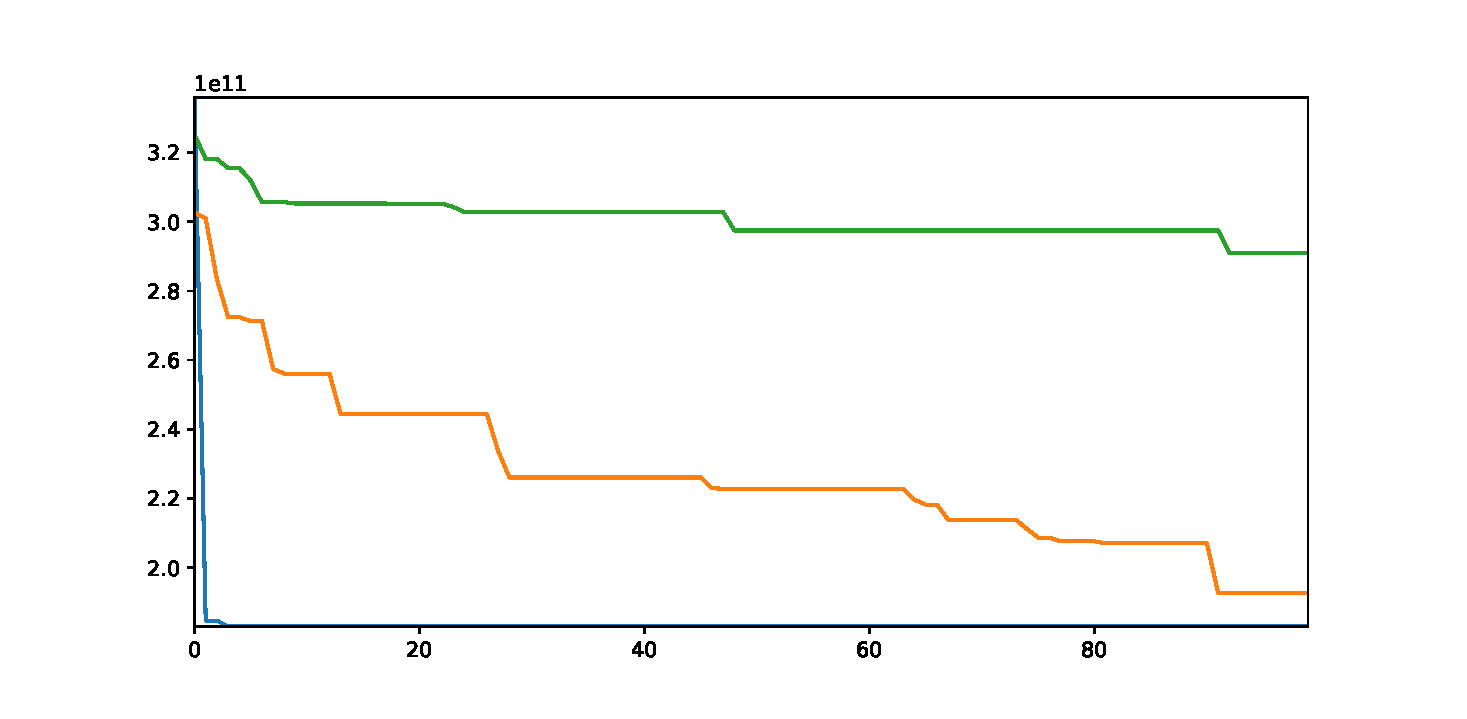
\includegraphics[scale=0.6]{cec2013_1.eps}
	\caption{optimization results for function no 2 from CEC 2013}
\end{figure}

\begin{figure}[H]
	\centering
	\includegraphics[scale=0.6]{cec2013_2.eps}
	\caption{optimization results for function no 5 from CEC 2013}
\end{figure}

\begin{figure}[H]
	\centering
	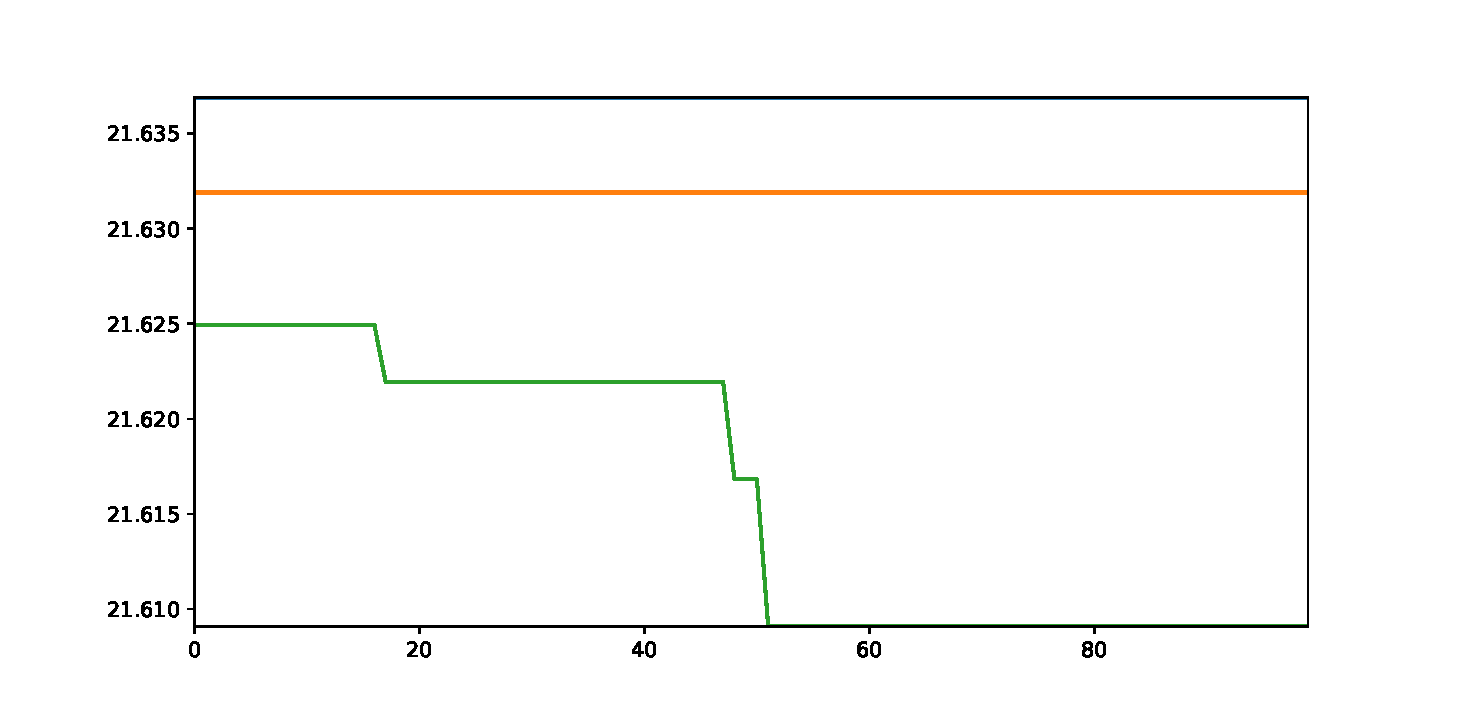
\includegraphics[scale=0.6]{cec2013_3.eps}
	\caption{optimization results for function no 7 from CEC 2013}
\end{figure}

\begin{figure}[H]
	\centering
	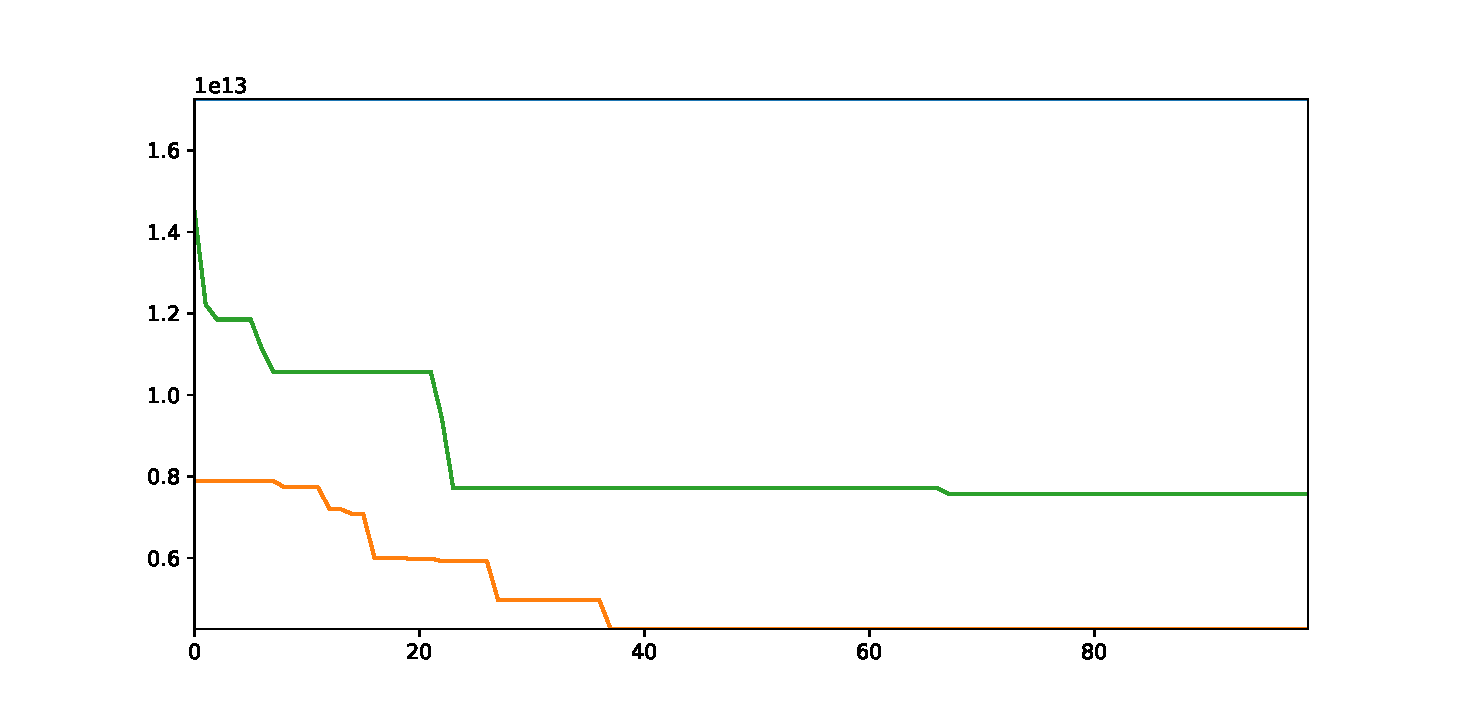
\includegraphics[scale=0.6]{cec2013_4.eps}
	\caption{optimization results for function no 14 from CEC 2013}
\end{figure}

\subsection{Other benchmarks}\label{subsec:other_testing}
TODO

\end{document}
